%!TEX root = thesis.tex


\begin{figure}
    \centering
    \scalebox{0.8}{
    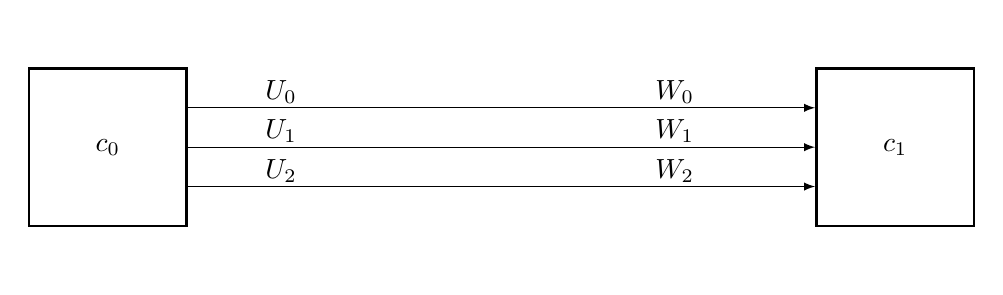
\begin{tikzpicture}
        [
            square/.style = {draw, shape=rectangle, minimum height=2cm, minimum width=2cm, node distance=2cm, line width=1pt},
            empty/.style = {draw, shape=rectangle, minimum height=2cm, minimum width=2cm, node distance=2cm, line width=1pt, draw=white},
        ]

        \node[empty] (0a) at (0,0.5)     {};
        \node[empty] (0b) at (0,-0.5)     {};
        \node[square] (0c) at (0,0)     {$c_0$};

        \node[empty] (1a) at (10cm,0.5)   {};
        \node[empty] (1b) at (10cm,-0.5)   {};
        \node[square] (1c) at (10cm,0)   {$c_1$};

        \node (x0) at (2.2cm,0.7) {$U_0$};
        \node (y0) at (2.2cm,-0.3) {$U_2$};
        \node (z0) at (2.2cm,0.2) {$U_1$};

        \node (x1) at (7.2cm,0.7) {$W_0$};
        \node (y1) at (7.2cm,-0.3) {$W_2$};
        \node (z1) at (7.2cm,0.2) {$W_1$};

        \draw [-latex] (0a.east) -- (1a.west);
        \draw [-latex] (0b.east) -- (1b.west);
        \draw [-latex] (0c.east) -- (1c.west);
    \end{tikzpicture}

}
\end{figure}
